\chapter{Tópicos de Gerência de Requisitos}
\label{management}

\section{Rastreabilidade}

\subsection{Introdução ao Conceito de Rastreabilidade}

A rastreabilidade advém da necessidade de identificar as dependências entre os artefatos, já que eles relacionam-se e afetam-se ao longo do desenvolvimento do \textit{software}. É notável que os requisitos mantém também dependência entre si de forma que alguns só podem ser implementados após outros. Sendo assim, é necessário identificar e controlar essas relações entre os requisitos com o intuito de evitar possíveis erros catastróficos e complicações para o desenvolvimento. A rastreabilidade é precisamente o que permite obter essa identificação e controle.

~\cite{gotel} definem a rastreabilidade de requisitos como “a capacidade de descrever e seguir a vida de um requisito, em ambas as direções para frente e para trás(\textit{forward and backward direction}), isso é, desde as suas origens, através do seu desenvolvimento e especificação, à sua subsequente implementação e utilização”.

Rastrear um requisito para frente (\textit{forward traceability}) significa “seguir as ligações de rastreabilidade para os artefatos que foram derivados do artefacto em consideração”.~\cite{winkler}

Rastrear um requisito para trás (\textit{backward traceability}) “refere-se à capacidade de seguir as ligações de rastreabilidade de um artefato específico de volta às suas origens de onde foi derivado”.~\cite{winkler}

A figura \ref{back-and-foward} demonstra as pré-rastreabilidades e pós-rastreabilidades, introduzidas por ~\cite{gotel}.

\begin{figure}[htb]
\centering
  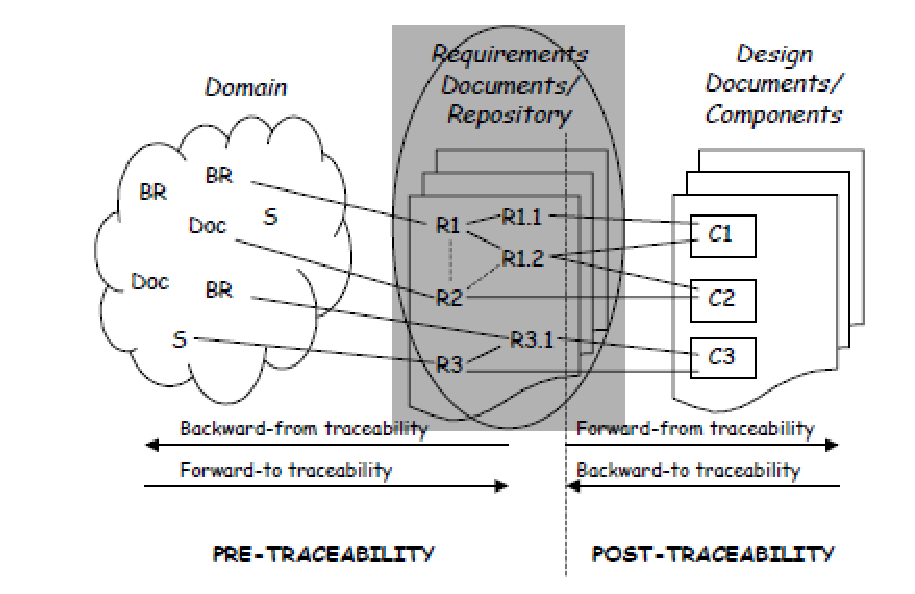
\includegraphics[keepaspectratio=true,scale=0.5]
  {figuras/rastreabilidade_frente_tras.eps}
  \caption{Rastreabilidade pra frente e pra trás ~\cite{dahlstedt}}
  \label{back-and-foward}
\end{figure}

\clearpage{}

\textbf{Pré-rastreabilidade}: “refere-se aos aspetos da existência de um requisito antes de ser incluído na especificação de requisitos” ~\cite{gotel} e “está focada em permitir uma melhor compreensão dos requisitos” ~\cite{persson}. “A pré-rastreabilidade é a base para gerir a evolução de um sistema, porque permite o levantamento das partes de especificação que são afetadas por uma mudança específica no pedido suscitado”.~\cite{persson}

\textbf{Pós-rastreabilidade}: “refere-se aos aspetos da existência de um requisito a partir do momento em que foi incluído na especificação de requisitos” ~\cite{gotel} e “está focada em permitir uma melhor compreensão e aceitação do atual \textit{software} de sistema”. ~\cite{persson}

Dentre os estudos da rastreabilidade de \textit{software}, ~\cite{ramesh} introduziram a rastreabilidade horizontal e vertical.

\begin{figure}[htb]
\centering
  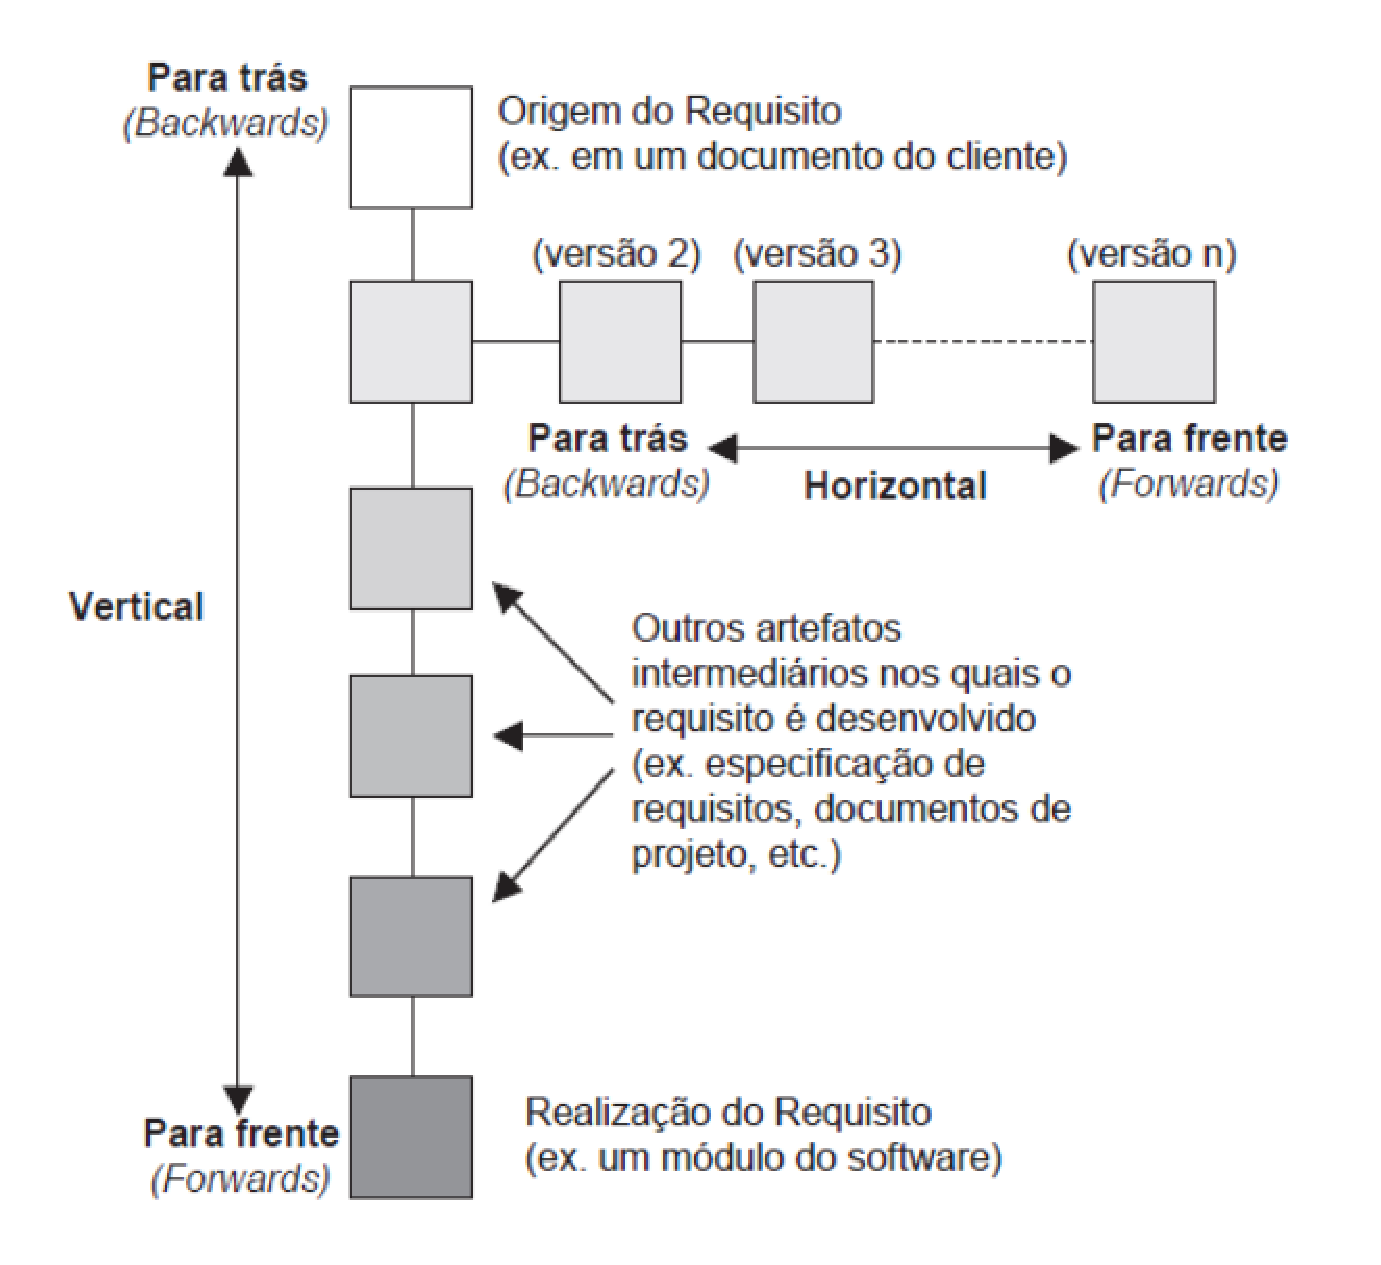
\includegraphics[keepaspectratio=true,scale=0.5]
  {figuras/rastreabilidade_horizontal.eps}
  \caption{Rastreabilidade horizontal e vertical ~\cite{genvigir}}
  \label{sideways}
\end{figure}

\clearpage{}


\textbf{Rastreabilidade Horizontal}: trata de relacionar versões ou variantes do mesmo tipo de informação, por exemplo, entre requisitos ou entre componentes do sistema. ~\cite{persson}~\cite{winkler}

\textbf{Rastreabilidade Vertical}: preocupa-se em rastrear informação entre anteriores e subsequentes fases no processo de desenvolvimento, isto é, entre objetos de informação de diferentes tipos ~\cite{persson}~\cite{winkler}. Por exemplo, uma relação entre um requisito e um elemento da conceção.~\cite{winkler}

\subsection{Sobre a Rastreabilidade no RUP}

Pelo própria definição de rastreabilidade do processo unificado: “A rastreabilidade é a capacidade de rastrear um elemento de projeto para outros elementos de projeto relacionados, especialmente aqueles relacionados a requisitos. Os elementos de projeto envolvidos na rastreabilidade são chamados de itens de rastreabilidade.  Os itens de rastreabilidade típicos incluem diferentes tipos de requisitos, elementos de modelo de análise e \textit{design}, produtos de trabalho de teste e materiais de treinamento e documentação de suporte ao usuário final”.~\cite{rup1}

A figura \ref{common-itens} a seguir demonstra esses itens comummente utilizados na rastreabilidade de um \textit{software}.

\begin{figure}[htb]
\centering
  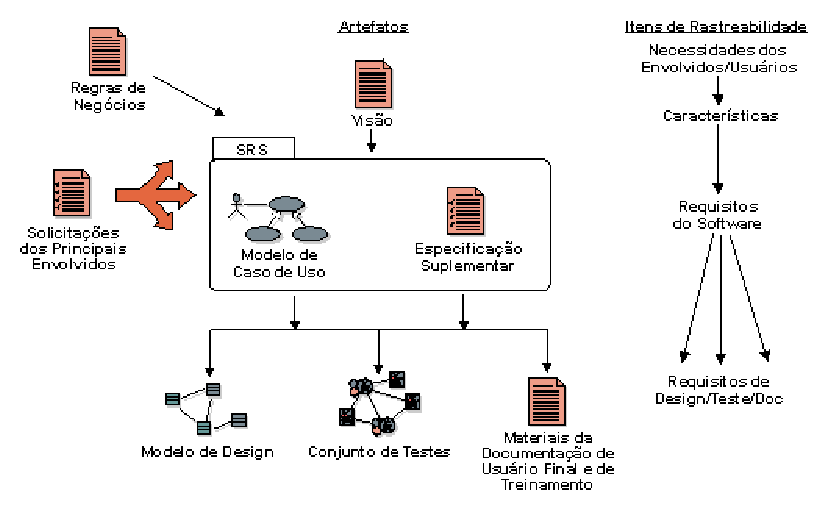
\includegraphics[keepaspectratio=true,scale=0.7]
  {figuras/itens_comuns.eps}
  \caption{Itens comumente utilizados na rastreabilidade.~\cite{rup1}}
  \label{common-itens}
\end{figure}

\clearpage{}


Os itens tipicamente utilizados são:

\begin{itemize}
\item Necessidades dos envolvidos, documentados no Documento de Visão.
\item Recurso do produto, documentados no Documento de Visão.
\item Requisito suplementar, documentados em Especificações Suplementares.
\item Casos de uso, documentados no Documento de Casos de Uso.
\item Seção de caso de uso, documentados no Documento de Casos de Uso.
\item Elemento de Design documentados no documento de Modelo de \textit{Design}.
\item Conjunto de Teste, documentados no documento de Caso de Teste.
\end{itemize}

Uma rastreabilidade típica pode ser vista pela figura \ref{common-tracebility} abaixo:

\begin{figure}[htb]
\centering
  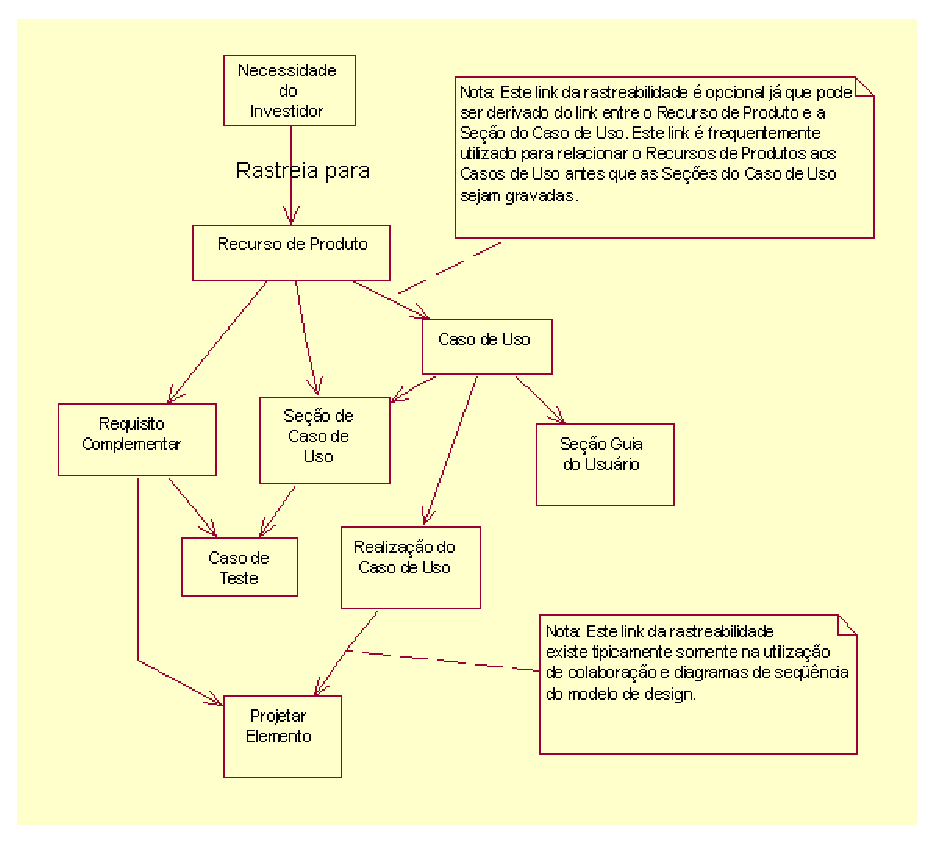
\includegraphics[keepaspectratio=true,scale=0.9]
  {figuras/rastreabilidade_tipica.eps}
  \caption{Rastreabilidade típica utilizada no RUP.~\cite{rup1}}
  \label{common-tracebility}
\end{figure}

\clearpage{}

Existem várias técnicas para realizar a rastreabilidade no processo unificado, dentre as mais comuns estão as referências cruzadas e o uso de documentos. As técnicas que utilizam as referências cruzadas são mais simples de serem implementadas e compreendidas, podendo utilizar numerações, indexação, \textit{tags} e matrizes de rastreabilidade. Já as técnicas que utilizam documentos, costumam usar \textit{templates} para os documentos e artefatos.

No caso de referências cruzadas, pode-se utilizar uma matriz de rastreabilidade, gerada por um \textit{software} de uso geral como uma planilha no Excel® ou em um \textit{software} específico como o Rational® RequisitePro®. Um exemplo de matriz de rastreabilidade pode ser visto pela tabela \ref{table1}.

\begin{table}[h]
\centering
\begin{tabular}{|l|l|l|l|l|}
\hline
\multicolumn{5}{|c|}{\textbf{Projeto \textless nome\textgreater - Matriz de Rastreabilidade}}           \\ \hline
\textbf{Requisito} & \textbf{Documento Fonte} & \multicolumn{1}{l|}{\textbf{Arquitetura}} & \textbf{Componente} & \textbf{Caso de Teste} \\ \hline
                   &                 &                                  &            &               \\ \hline
                   &                 &                                  &            &               \\ \hline
\end{tabular}
\caption{Rastreabilidade entre requisitos e seus correspondentes artefatos gerados}
\label{table1}
\end{table}

O requisito pode ser expresso em linguagem natural e numerado sequencialmente. Nas demais colunas, são indicados os artefatos relacionados ao requisito, onde a ordem correspondente é sempre de 1 para 1.

A mesma técnica pode ser utilizada para referenciar dependência entre requisitos, como pode ser observado pela figura \ref{matrix_requirement}.

\begin{figure}[htb]
\centering
  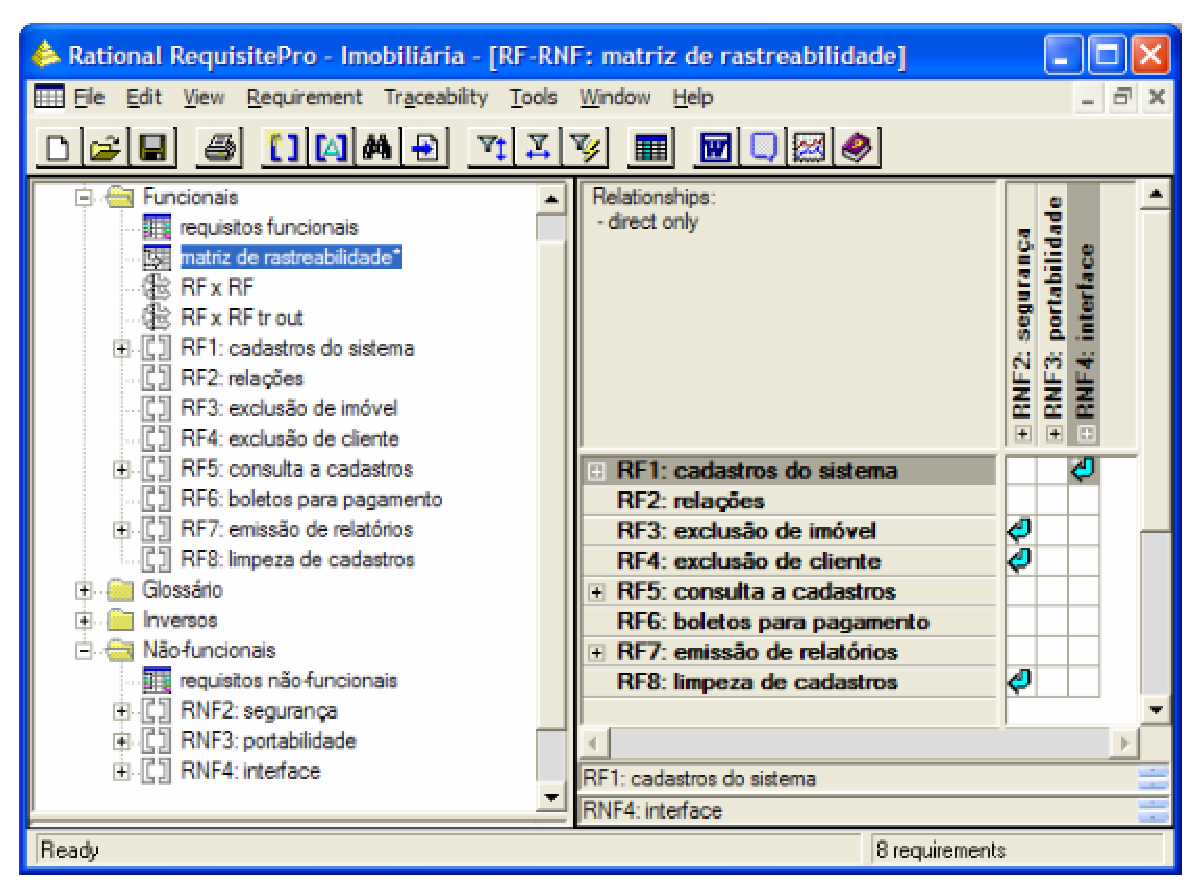
\includegraphics[keepaspectratio=true,scale=0.7]
  {figuras/matriz_rastreabilidade2.eps}
  \caption{Matriz de  rastreabilidade  entre  Requisitos  Funcionais  e  Não Funcionais.}
  \label{matrix_requirement}
\end{figure}

\clearpage{}

\subsection{Rastreabilidade Adotada no Projeto}

Considerando a necessidade de cada requisito ser rastreável à sua fonte e seu uso durante o projeto em implementações e testes, por exemplo, foi escolhido a utilização da rastreabilidade vertical especificada abaixo.

Distribuição dos artefatos gerados:

\begin{figure}[htb]
\centering
  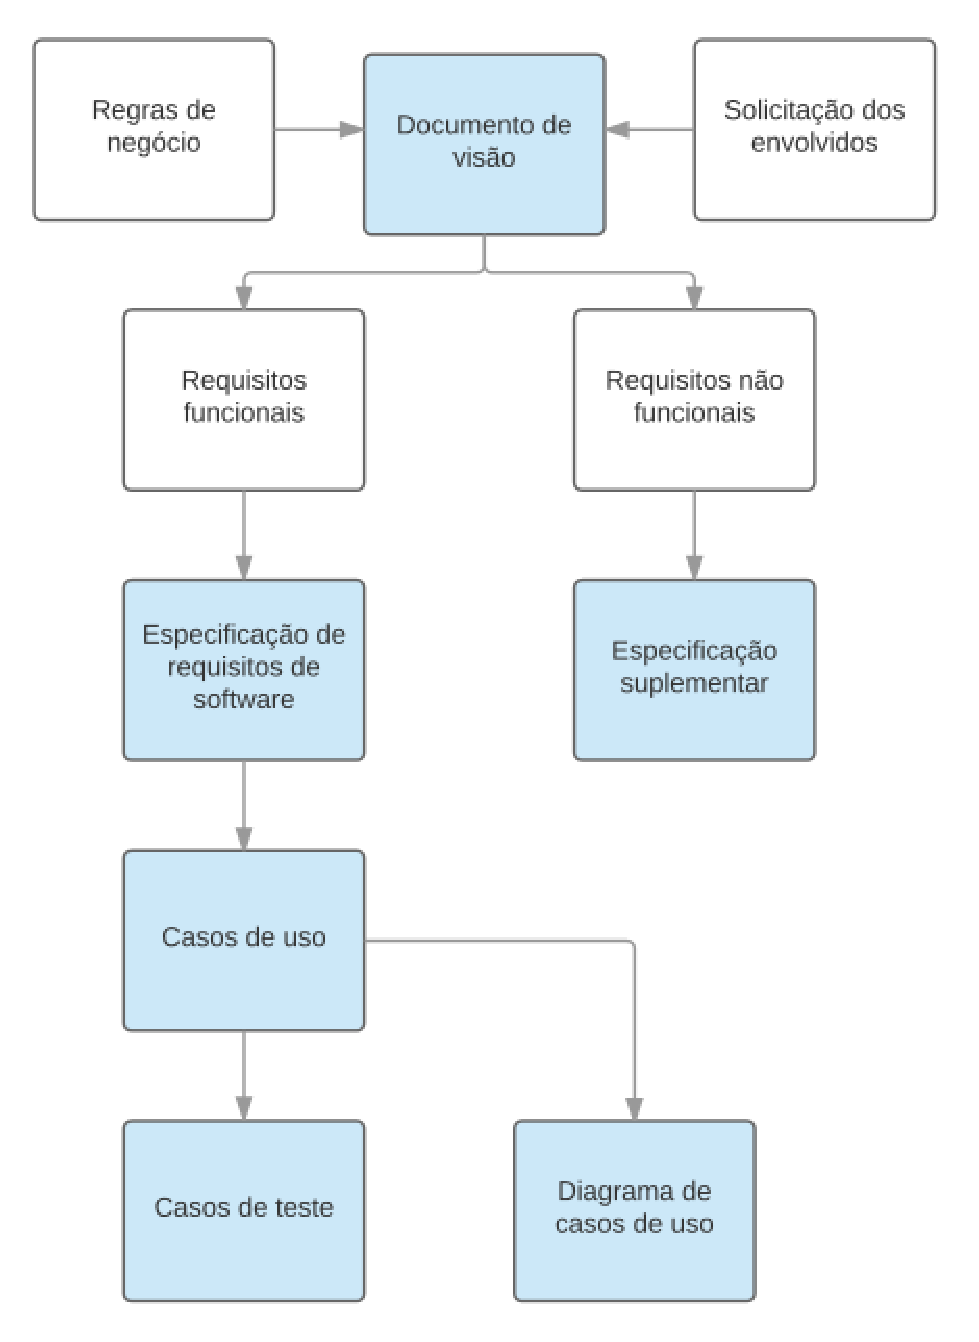
\includegraphics[keepaspectratio=true,scale=0.7]
  {figuras/arvore_rastreabilidade.eps}
  \caption{Árvore de rastreabilidade}
  \label{matrix_requirement}
\end{figure}

Identificação dos itens dos artefatos:

\begin{table}[]
\centering
\label{artefacts-identifier}
\begin{tabular}{|l|l|}
\hline
\textbf{Identificador}         & \textbf{Descrição}                  \\ \hline
RN\textless número\textgreater  & Regra de Negócio                    \\ \hline
RF\textless número\textgreater  & Requisito Funcional. Ex: RF0014     \\ \hline
RNF\textless número\textgreater & Requisito Não Funcional. EX:RNF0365 \\ \hline
UC\textless número\textgreater  & Caso de Uso. Ex:US1234              \\ \hline
UCD\textless número\textgreater & Diagrama de Caso de Uso             \\ \hline
TC\textless número \textgreater  & Caso de Teste.                     \\ \hline
\end{tabular}
\caption{Identificação dos artefatos}
\end{table}

\begin{itemize}
\item \textbf{Atributos de Requisitos}: Características utilizadas para avaliar um requisito. Serão utilizados:

\begin{itemize}
\item Prioridade
\item \textit Status
\item Dificuldade
\end{itemize}

\item \textbf{Prioridade}: Define o quão importante é o requisito para o sistema em relação aos demais. Os de maior prioridade serão implementados antes em relação aos demais, isso para todos os níveis de prioridade, que são:

\begin{itemize}
\item Alta
\item Média
\item Baixa
\end{itemize}

\item \textbf{\textit{Status}}: Seguindo o mesmo exemplo de prioridade, em \textit{status} também serão utilizados 3 níveis que dirão o progresso das atividades relacionadas à um requisito:

\begin{itemize}
\item Completado
\item Em andamento
\item Não inicializado
\end{itemize}

\item \textbf{Dificuldade}: Serve de indicativo para uma possível dificuldade na implementação dos requisitos. É um atributo fundamental para o planejamento das iterações. Também será dividido em 3 níveis:

\begin{itemize}
\item Alta
\item Média
\item Baixa
\end{itemize}
\end{itemize}

Para servir de exemplo, segue-se uma tabela de atributos:

\begin{table}[h]
\centering
\label{requirements-qualities}
\begin{tabular}{|l|l|l|l|l|}
\hline
\textbf{Identificador} & \textbf{Nome} & \textbf{Prioridade} & \textbf{Dificuldade} & \textbf{Status} \\ \hline
                       &               &                     &                      &                 \\ \hline
\end{tabular}
\caption{Atributos dos Requisitos}
\end{table}

Para ter um maior controle sobre o fluxo do relacionamento entre os artefatos e os requisitos, será utilizada uma matriz de rastreabilidade como o modelo abaixo:

\begin{table}[h]
\centering
\label{itens-traceability}
\begin{tabular}{|l|l|l|l|l|}
\hline
\multicolumn{5}{|c|}{\textbf{Alvos}}                  \\ \hline
\multirow{4}{*}{\textbf{Fontes}} & F/A & A1 & A2 & A3 \\ \cline{2-5} 
                                 & F1  & X  &    & X  \\ \cline{2-5} 
                                 & F2  &    & X  &    \\ \cline{2-5} 
                                 & F3  &    &    & X  \\ \hline
\end{tabular}
\caption{Modelo de como será a disposição dos itens na matriz de rastreabilidade}
\end{table}

Segue um exemplo também de uma matriz de rastreabilidade entre casos de uso e requisitos:

\begin{figure}[htb]
\centering
  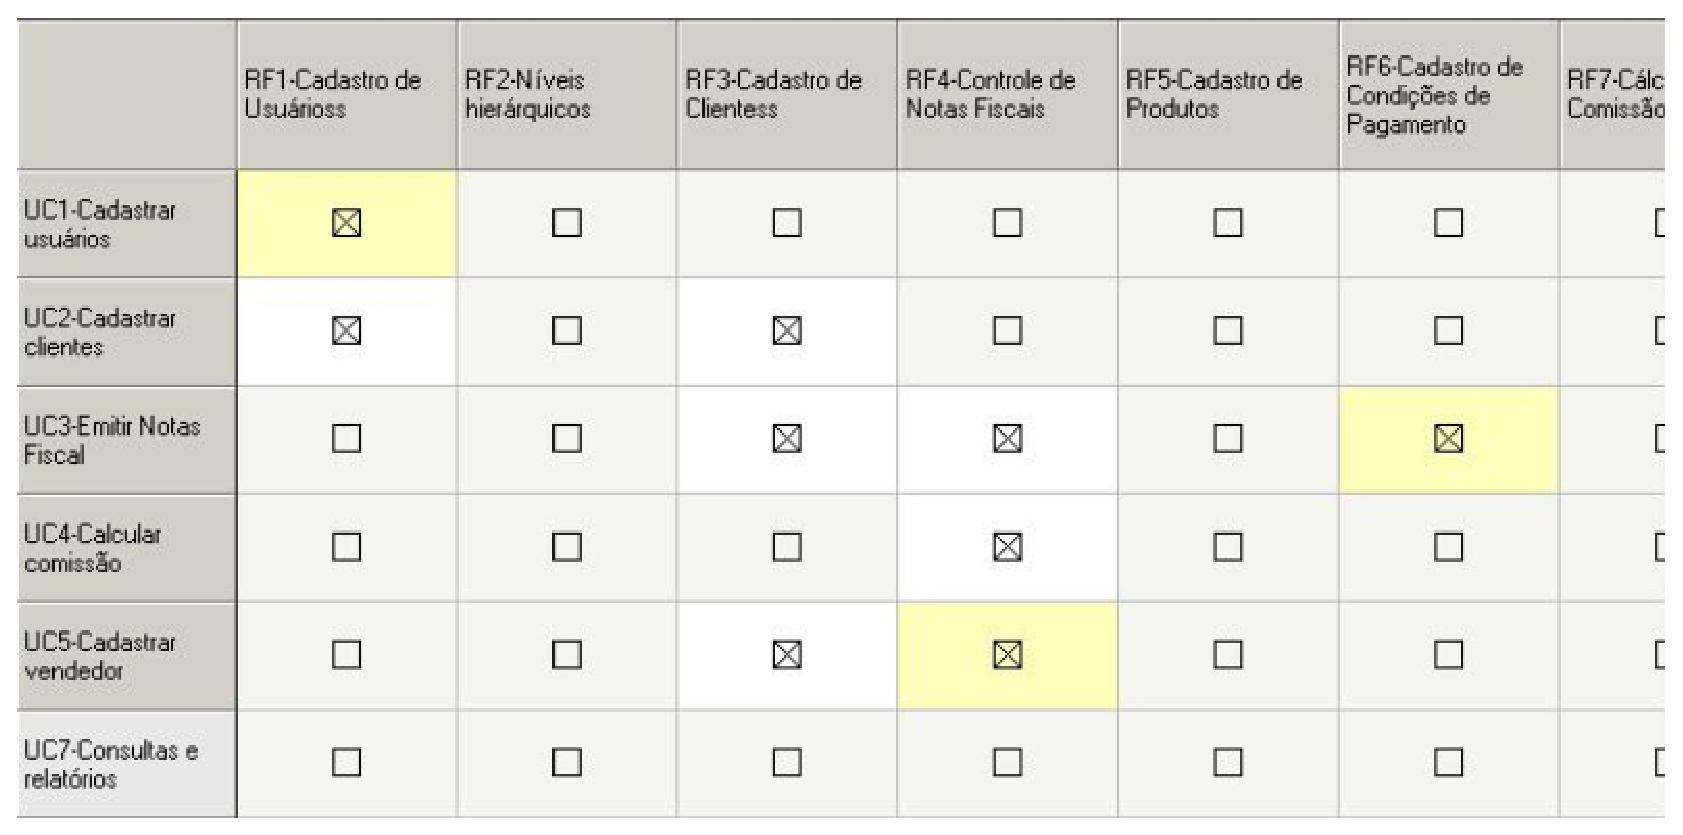
\includegraphics[keepaspectratio=true,scale=0.5]
  {figuras/casos_de_uso.eps}
  \caption{Casos de Uso e Requisitos.~\cite{dev1}}
  \label{uc-requirements}
\end{figure}

\section{Modelos de Maturidade}

\subsection{Introdução à Modelos de Maturidade}

Um modelo de maturidade é responsável por analisar e avaliar cada processo de uma estrutura organizacional de forma a melhorar o mesmo em cada nível da empresa avaliada. Em outras palavras, ele é responsável por avaliar a capacidade de processos na realização de seus objetivos, localizar oportunidades de melhoria de produtividade, redução de custos e planejar e monitorar as ações de melhoria contínua dos processos empresariais.

\subsection{CMMI}

“O CMMI é uma metodologia criada pela \textit{Software Engineering Institute} (SEI) para ser um guia destinado a melhorar os processos organizacionais e habilidade desses em gerenciar o desenvolvimento, a aquisição e a manutenção de produtos e serviços. O CMMI organiza as práticas, que já são consideradas efetivas, em uma estrutura que visa auxiliar a organização a estabelecer prioridades para melhoria e também fornece um guia para a implementação dessas melhorias.”[1]
O CMMI traz consigo grandes possibilidades para melhoria em projetos, elevando o nível da qualidade e cumprindo melhor os prazos estipulados.
O CMMI se divide em 5 estágios:

\begin{itemize}
\item Otimização
\item Quantitativamente Gerenciado
\item Definido
\item Gerenciado
\item Inicial
\end{itemize}

Os níveis em que a engenharia de requisitos está presente são Gerenciado e Definido. Nesses níveis, a ER subdivide em 6 processos:

\begin{enumerate}
\item Gerência de Requisitos
\item Desenvolvimento de Requisitos
\item Solução Técnica
\item Integração do Produto
\item Verificação
\item Validação
\end{enumerate}

\subsubsection{Vantagens e Desvantagens}

\begin{itemize}
	\item Vantagens
		\begin{itemize}
			\item Reconhecimento internacional
			\item Eliminação de inconsistências
			\item Utilização de terminologia comum
			\item Desenvolvimento de \textit{software} com qualidade, garantindo cumprimento de prazos e atendendo às necessidades dos clientes 
			\item Consistência com a norma ISO-15504 (norma que define o processo de desenvolvimento de \textit{software} de acordo com os níveis de capacidade para cada processo de acordo com o CMMI (CORTES, 2004)
			\item Integração de sistemas
			\item Métricas e análises
			\item Identificação de riscos
		\end{itemize}
	\item Desvantagens
		\begin{itemize}
			\item Não há nenhuma empresa brasileira certificada pelo SEI para auditoria, sendo necessário que a certificação seja criada nos Estados Unidos e trazida por um \textit{lead assessor}
			\item Os preços de avaliação do CMMI podem variar de 36 a 60 mil dólares. Se a empresa necessitar de assessoria, o preço pode chegar à cerca de 125 mil dólares por ano (CMMI, 2015). Por esse motivo, pequenas e médias empresas tem problema em adotar esse modelo.
		\end{itemize}
\end{itemize}

\subsection{MPS-BR}

“É um movimento de melhoria de software voltado para a realidade brasileira. O programa é coordenado pela Associação para promoção de Software brasileiro (SOFTEX) com início de desenvolvimento em 2003.”~\cite{softex}

É voltado para a realidade brasileira, 	além disso, é adequado para micro, pequenas e medias empresas alcançarem melhorias no processo de construção de um software.

Os níveis definidos no MPS-BR são:

\begin{itemize}
	\item A - Em otimização
	\item B - Gerenciado Quantitativamente
	\item C - Definido
	\item D - Largamento Definido
	\item E - Parcialmente Definido
	\item F - Gerenciado
	\item G - Parcialmente Gerenciado
\end{itemize}

O foco da ER está nos níveis G e D.

\subsubsection{Vantagens e Desvantagens}

\begin{itemize}
	\item Vantagens
		\begin{itemize}
			\item Adequado à realidade brasileira (implementação acessível à micro, pequenas e médias empresas)
			\item Possui compatibilidade com o CMMI (baseado nas normas ISO 12207 e 15504)
			\item Integração universidade-empresa
			\item Avaliações feitas por empresas brasileiras
			\item Custo relativamente pequeno (cerca de 72 mil reais para uma empresa nível G ser habilitada como nível F)
			\item Avaliação rápida (feitas em até 5 dias)
		\end{itemize}
	\item Desvantagens
		\begin{itemize}
			\item A certificação não é competitiva o suficiente para tornar a empresa reconhecida internacionalmente
			\item Foco principal em pequenas empresas
		\end{itemize}
\end{itemize}

\subsection{Por que utilizar o MPS-BR para modelar o processo da Engrena?}

Enquanto o CMMI oferece competitividade e reconhecimento internacional, ele é um modelo extremamente caro para utilizar em um ambiente de Empresa Júnior.
Já o MPS-BR é adaptado à realidade brasileira, facilitando a implementação gradual dos processos de gerência, focado na gerência de requisitos e desenvolvimento de requisitos. Implementação essa que conta com preços mais acessíveis e objetivos esperados, com divisões claras que facilitam a visibilidade dos resultados da melhoria de processos em prazos mais curtos.
